\chapter{Results}
TODO AGGIUNGERE

\section{Graph-based Framework}
The OoM was classified using three distinct features: speed, acceleration and angular momentum, as described in Section \ref{subsec:alg_features}.
For each feature, we calculated the accuracy of the method in predicting the correct edge compared to the true label.\\
In Table \ref{tab:clust_results} we can see the results.

\begin{table}[H]
  \centering
  \begin{tabular}{||>{\centering\arraybackslash}p{1.2cm}||>{\centering\arraybackslash}p{4.3cm}||>{\centering\arraybackslash}p{4.3cm}||>{\centering\arraybackslash}p{4.3cm}||}
  \hline
  & \textbf{Speed} & \textbf{Acceleration} & \textbf{Angular Momentum} \\
  \hline
  \textbf{WDG} & 28.3\%  & 26.7\%  & 36.6\%  \\
  \hline
  \end{tabular}
  \caption{Classification accuracy with WDC on the overall dataset}
  \label{tab:clust_results}
\end{table}

Even though these results are not impressive, they are still better than a random approach, where two random nodes are selected, and by examining which edges in the auxiliary graph they are connected to, they are compared to the ground truth. \\
Such an approach, in fact, achieves an accuracy of 19\%.
Figure \ref{fig:wdc_results} shows the distribution of the results for each edge of the dataset:
\begin{figure}
  \centering
  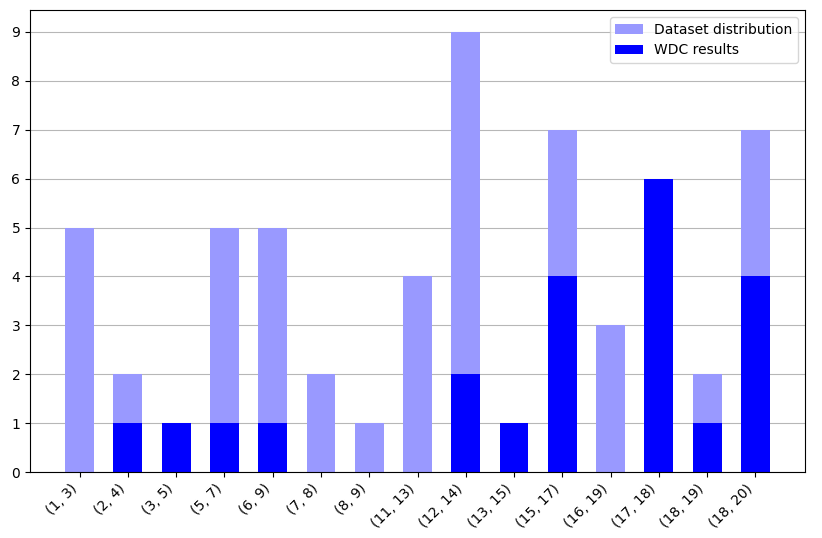
\includegraphics[width=0.85\textwidth]{wdc_results.png}
  \caption{Joints and frequency of the dataset and the correctly classified WDC algorithm}
  \label{fig:wdc_results}
\end{figure}

\clearpage

\section{Clusters Stabilization}
In this first example, in Figure \ref{fig:stabilization_results}, we can observe the results of stabilization between two different instants in time. 
In (a), the preceding time instant is visible, while (b) showcases the subsequent time instant in an unstabilized state. 
In (c) instead, the subsequent time instant with clusters stabilized.
\begin{figure}[H]
  \centering
  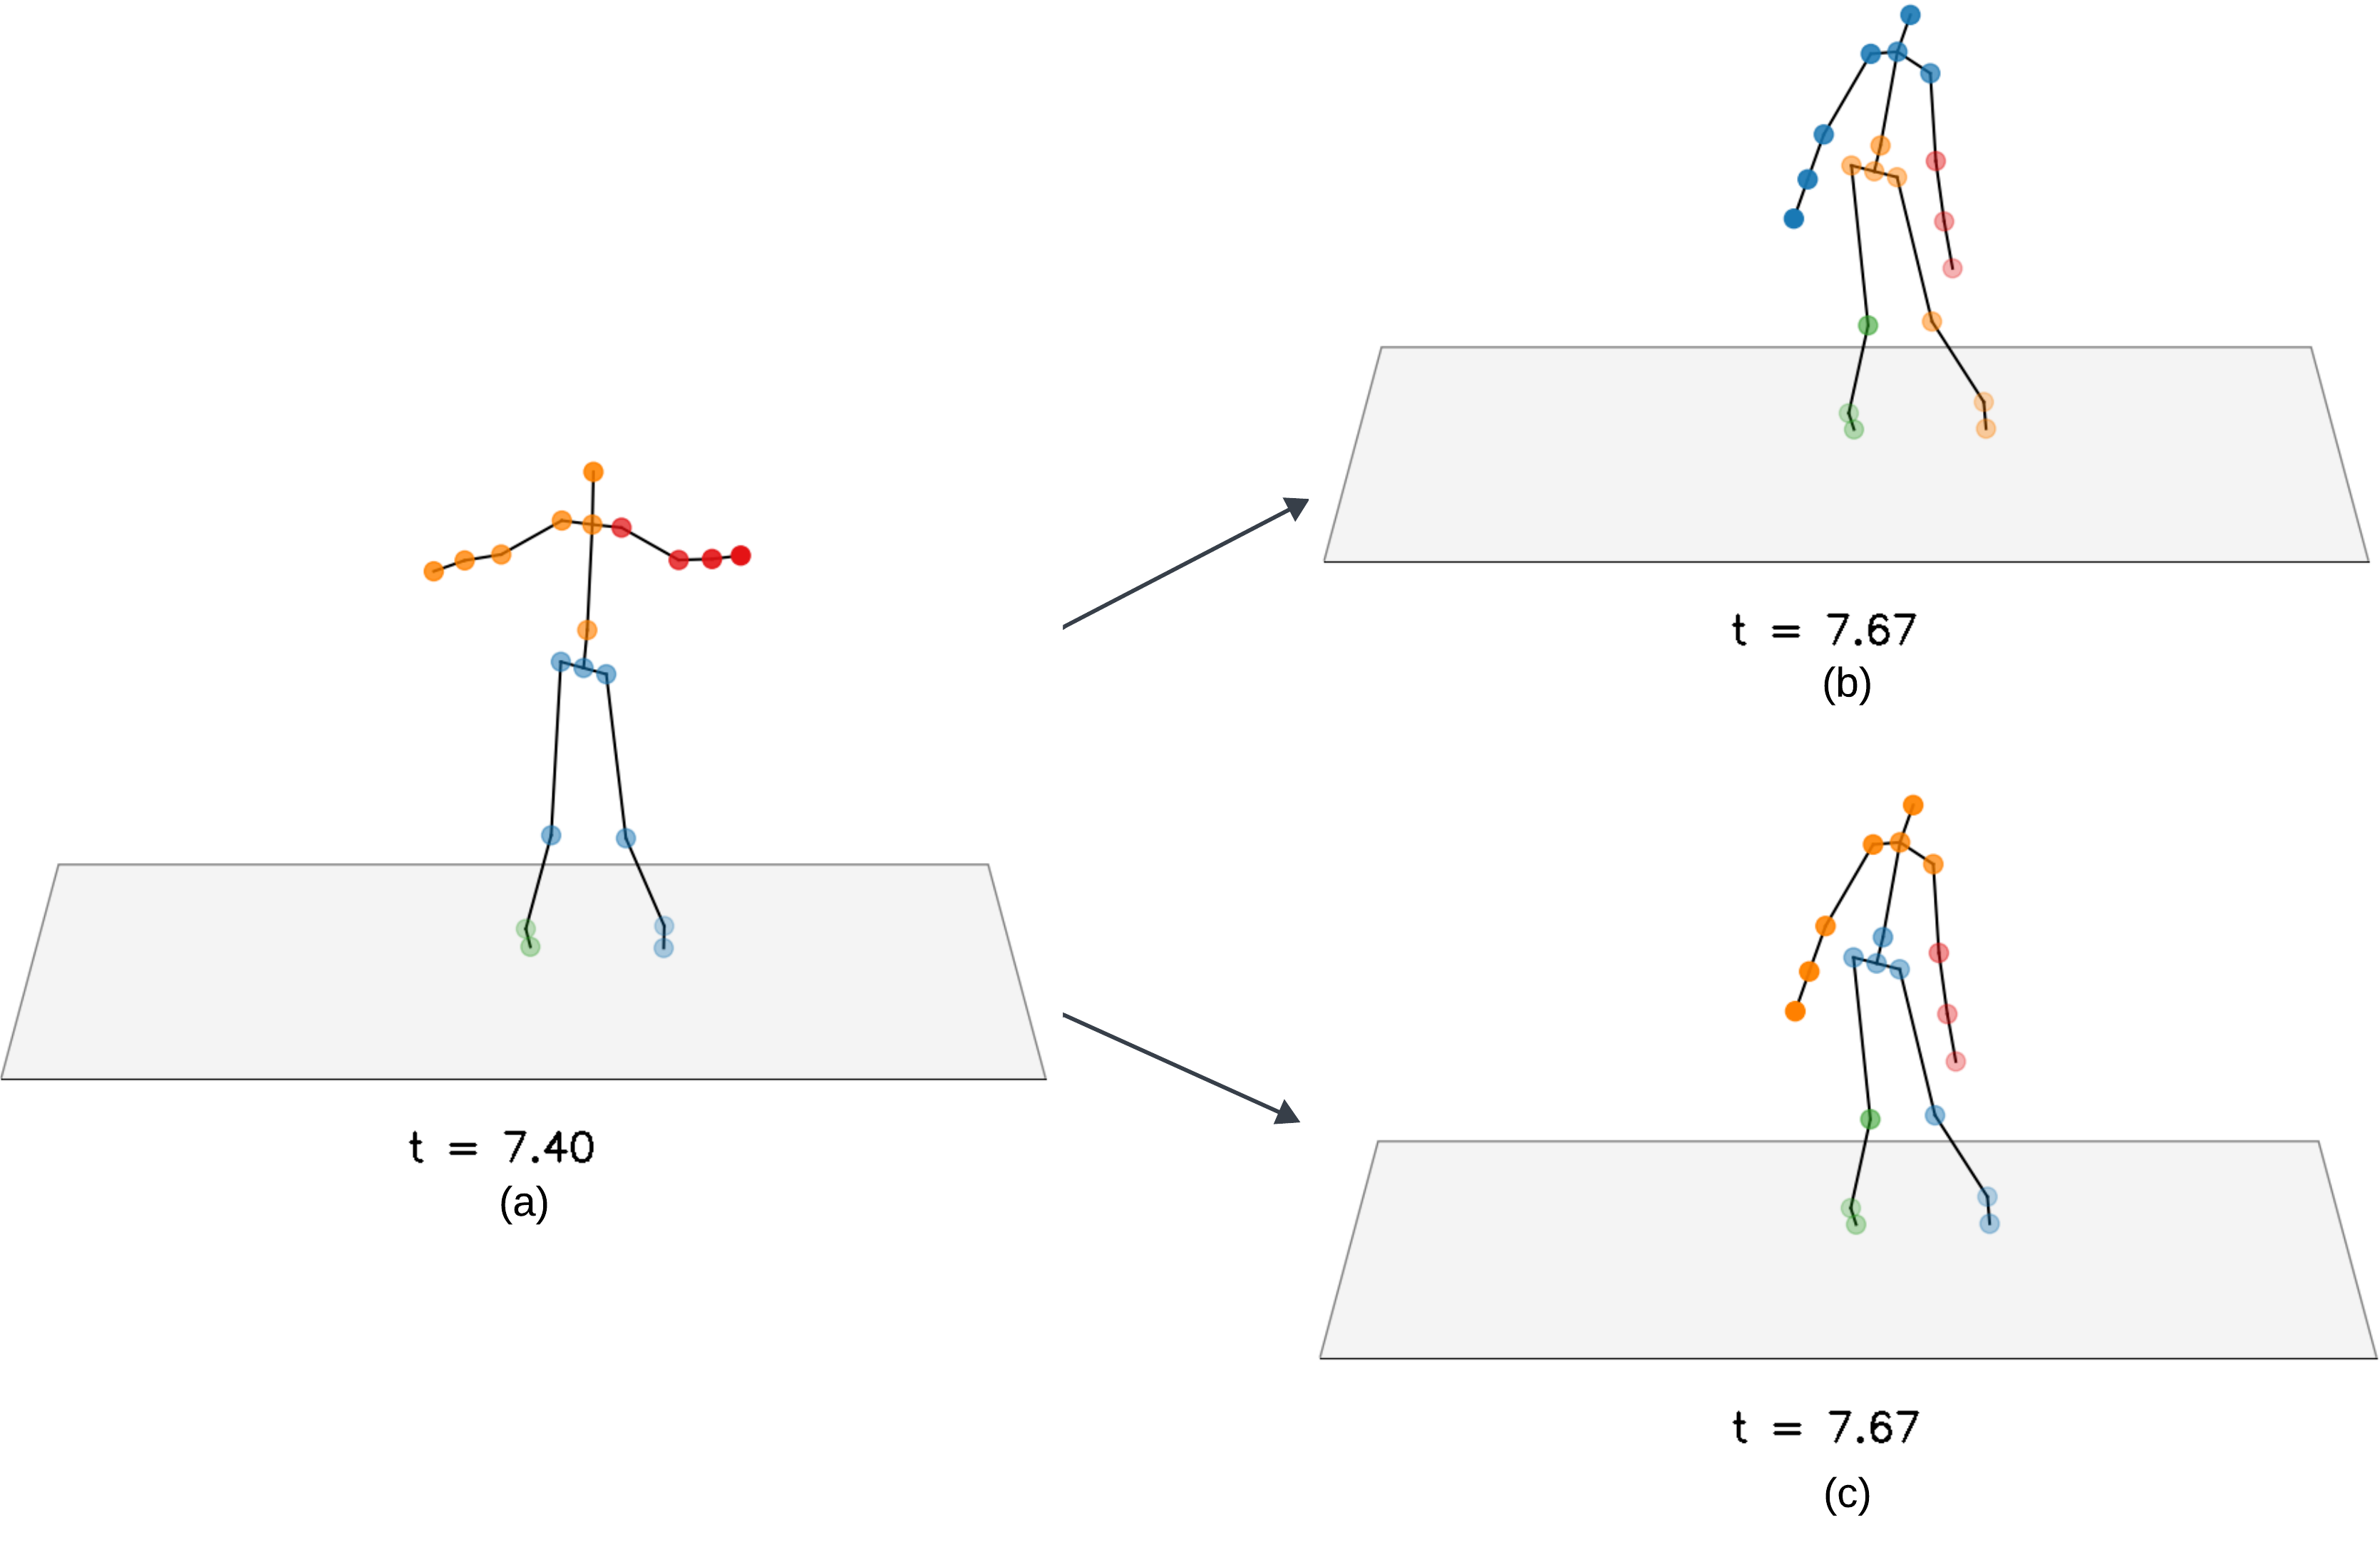
\includegraphics[width=0.9\textwidth]{ClustersStabilization.png}
  \caption{Clustering at $t=7.40$ (a), $t=7.67$ unstabilized (b), and $t=7.67$ stabilized (c).}
  \label{fig:stabilization_results}
\end{figure}

For a comprehensive view of the stabilization outcomes, reference the QR code in Figure \ref{fig:QRcode}. 
This code leads to a GIF image showcasing the entire motion sequence.
\begin{figure}[H]
  \centering
  
\includegraphics[width=0.50\textwidth]{qrcode.png}
  \caption{QRcode to the GIF}
  \label{fig:QRcode}
\end{figure}

As evident from the GIF, the dancer begins from a stance with slightly spread legs and the left arm raised upwards.
Throughout the movement, the left arm descends while moving backward, the torso leans forward, taking the right arm along with it, and the left foot lifts off the ground, taking a step backward.

\clearpage

\section{Machine Learning}
In the following Tables (from \ref{tab:ml_results_cm_joints} to \ref{tab:ml_results_cm_body_parts}), you will find confusion matrices and evaluation metrics for the prediction of certain classes.
To interpret the meaning of the confusion matrices, please refer to Section \ref{subsec:evaluation_metrics}.
\\

The tests to identify the best model were conducted on the most frequent edge of the dataset, \textit{left\_hand - left\_wrist} with the aim of maximize the accuracy.
This is because the dataset is unbalanced, and therefore, better prediction results are expected from this class.
As observed, accuracy consistently remains very high, almost always exceeding 70\%.
However, beyond this, the model demonstrates high $specificity$, meaning it excels at maximizing TN but struggles to identify TP effectively.
This behavior is evident in the TPR, which varies significantly across different classes.
The model requires a high level of certainty in predictions before classifying a sample as positive.
You can also observe the model's high specificity from the TNR, which is consistently quite high in all cases, typically greater than 80\%. \\
In summary, the model tends to favor a conservative strategy, prioritizing the reduction of FP, leading to a high specificity but limited effectiveness in identifying TP.

\clearpage
\begin{table}[H]
    \centering
    \renewcommand{\arraystretch}{1.2} % Aumenta lo spazio tra le righe del doppio
    \begin{subfigure}[b]{0.1\textwidth}
        \centering
        \begin{tabular}{|>{\centering\arraybackslash}p{0.5cm}|>{\centering\arraybackslash}p{0.5cm}|}
        \hline
        48 & 3 \\
        \hline
        3 & 6 \\
        \hline
        \end{tabular}
        \caption{}
        \label{tab:ml_results_cm_edge_1}
    \end{subfigure}
    \hspace{0.05\linewidth}
    \begin{subfigure}[b]{0.1\textwidth}
        \centering
        \begin{tabular}{|>{\centering\arraybackslash}p{0.5cm}|>{\centering\arraybackslash}p{0.5cm}|}
        \hline
        51 & 2 \\
        \hline
        6 & 1 \\
        \hline
        \end{tabular}
        \caption{}
        \label{tab:ml_results_cm_edge_2}
    \end{subfigure}
    \hspace{0.05\linewidth}
    \begin{subfigure}[b]{0.1\textwidth}
        \centering
        \begin{tabular}{|>{\centering\arraybackslash}p{0.5cm}|>{\centering\arraybackslash}p{0.5cm}|}
        \hline
        44 & 9 \\
        \hline
        7 & 0 \\
        \hline
        \end{tabular}
        \caption{}
        \label{tab:ml_results_cm_edge_3}
    \end{subfigure}
    \hspace{0.05\linewidth}
    \begin{subfigure}[b]{0.1\textwidth}
        \centering
        \begin{tabular}{|>{\centering\arraybackslash}p{0.5cm}|>{\centering\arraybackslash}p{0.5cm}|}
        \hline
        51 & 3 \\
        \hline
        4 & 2\\
        \hline
        \end{tabular}
        \caption{}
        \label{tab:ml_results_cm_edge_4}
    \end{subfigure}
    \hspace{0.05\linewidth}
    \begin{subfigure}[b]{0.1\textwidth}
        \centering
        \begin{tabular}{|>{\centering\arraybackslash}p{0.5cm}|>{\centering\arraybackslash}p{0.5cm}|}
        \hline
        52 & 3 \\
        \hline
        4 & 1 \\
        \hline
        \end{tabular}
        \caption{}
        \label{tab:ml_results_cm_edge_5}
    \end{subfigure}
    \hspace{0.05\linewidth}
    \begin{subfigure}[b]{0.1\textwidth}
        \centering
        \begin{tabular}{|>{\centering\arraybackslash}p{0.5cm}|>{\centering\arraybackslash}p{0.5cm}|}
        \hline
        53 & 2 \\
        \hline
        2 & 3 \\
        \hline
        \end{tabular}
        \caption{}
        \label{tab:ml_results_cm_edge_6}
    \end{subfigure}
    \hspace{0.05\linewidth}
    \caption{Confusion matrices of the 6 most frequent classes in the dataset}
    \label{tab:ml_results_cm_joints}
\end{table}

%TODO AGGIUNGERE TOP FEATURES PER EXPLAINABILITY
\begin{table}[H]
    \centering
    \begin{tabular}{||>{\centering\arraybackslash}p{2cm}||>{\centering\arraybackslash}p{6cm}||>{\centering\arraybackslash}p{2cm}||>{\centering\arraybackslash}p{2cm}||>{\centering\arraybackslash}p{2cm}||}
    \hline
    \textbf{Label} & \textbf{Edge} & \textbf{TPR} & \textbf{TNR} &\textbf{Accuracy} \\
    \hline
    (a) & left\_hand - left\_wrist  & 66\% & 94\% & 90\% \\
    \hline
    (b) & shoulder\_center - head  & 14\% & 96\% & 87\% \\
    \hline
    (c) & right\_elbow - right\_shoulder  & 0\%  & 83\% & 73\% \\ 
    \hline
    (d) & right\_shoulder - shoulder\_center & 33\% & 94\% & 88\% \\
    \hline
    (e) & right\_knee - right\_hip  & 20\%  & 95\% & 88\%\\
    \hline
    (f) & left\_knee - left\_hip  & 60\% & 96\% & 93\%\\ 
    \hline
    \end{tabular}
    \caption{Metrics of the 6 classes most frequent of the dataset}
    \label{tab:ml_results_joints}
\end{table}




\begin{table}[H]
  \begin{minipage}[b]{0.1\textwidth}
    \centering
    \renewcommand{\arraystretch}{1.2} % Aumenta lo spazio tra le righe del doppio
    \begin{tabular}{|>{\centering\arraybackslash}p{0.5cm}|>{\centering\arraybackslash}p{0.5cm}|}
    \hline
    37 & 5 \\
    \hline
    7 & 11 \\
    \hline
    \end{tabular}
    \caption*{(g)}
    \label{tab:ml_results_cm_body_part_1}
  \end{minipage}
  \hspace{0.05\linewidth}
  \begin{minipage}[b]{0.1\textwidth}
    \centering
    \renewcommand{\arraystretch}{1.2} % Aumenta lo spazio tra le righe del doppio
    \begin{tabular}{|>{\centering\arraybackslash}p{0.5cm}|>{\centering\arraybackslash}p{0.5cm}|}
    \hline
    37 & 9 \\
    \hline
    10 & 4 \\
    \hline
    \end{tabular}
    \caption*{(h)}
    \label{tab:ml_results_cm_body_part_2}
  \end{minipage}
  \hspace{0.05\linewidth}
  \begin{minipage}[b]{0.1\textwidth}
    \centering
    \renewcommand{\arraystretch}{1.2} % Aumenta lo spazio tra le righe del doppio
    \begin{tabular}{|>{\centering\arraybackslash}p{0.5cm}|>{\centering\arraybackslash}p{0.5cm}|}
    \hline
    43 & 4 \\
    \hline
    6 & 7 \\
    \hline
    \end{tabular}
    \caption*{(i)}
    \label{tab:ml_results_cm_body_part_3}
  \end{minipage}
  \hspace{0.05\linewidth}
  \begin{minipage}[b]{0.1\textwidth}
    \centering
    \renewcommand{\arraystretch}{1.2} % Aumenta lo spazio tra le righe del doppio
    \begin{tabular}{|>{\centering\arraybackslash}p{0.5cm}|>{\centering\arraybackslash}p{0.5cm}|}
    \hline
    47 & 5 \\
    \hline
    7 & 1\\
    \hline
    \end{tabular}
    \caption*{(l)}
    \label{tab:ml_results_cm_body_part_4}
  \end{minipage}
  \hspace{0.05\linewidth}
  \begin{minipage}[b]{0.1\textwidth}
    \centering
    \renewcommand{\arraystretch}{1.2} % Aumenta lo spazio tra le righe del doppio
    \begin{tabular}{|>{\centering\arraybackslash}p{0.5cm}|>{\centering\arraybackslash}p{0.5cm}|}
    \hline
    51 & 2 \\
    \hline
    6 & 1 \\
    \hline
    \end{tabular}
    \caption*{(m)}
    \label{tab:ml_results_cm_body_part_5}
  \end{minipage}
  \hspace{0.05\linewidth}
  \begin{minipage}[b]{0.1\textwidth}
    \centering
    \renewcommand{\arraystretch}{1.2} % Aumenta lo spazio tra le righe del doppio
    \begin{tabular}{|>{\centering\arraybackslash}p{0.5cm}|>{\centering\arraybackslash}p{0.5cm}|}
        \hline
        16 & 5 \\
        \hline
        8 & 31 \\
        \hline
    \end{tabular}
    \caption*{(n)}
    \label{tab:ml_results_cm_body_part_6}
  \end{minipage}
  \hfill
  \caption{Confusion matrices of the 5 Body Parts and of the Upper/Lower part}
  \label{tab:ml_results_cm_body_parts}
\end{table}


\begin{table}[H]
    \centering
    \begin{tabular}{||>{\centering\arraybackslash}p{2cm}||>{\centering\arraybackslash}p{6cm}||>{\centering\arraybackslash}p{2cm}||>{\centering\arraybackslash}p{2cm}||>{\centering\arraybackslash}p{2cm}||}
        \hline
        \textbf{Label} & \textbf{Body Part} & \textbf{TPR} & \textbf{TNR} & \textbf{Accuracy} \\
        \hline
        (g) & Right Arm  & 61\% & 88\% & 80\% \\
        \hline
        (h) & Left Arm & 29\% & 80\% & 68\% \\
        \hline
        (i) & Right Leg  & 54\%  & 91\% & 83\% \\ 
        \hline
        (l) & Left Leg & 12\% & 90\% & 80\% \\
        \hline
        (m) & Head  & 14\%  & 96\% & 86\%\\
        \hline
        \hline
    \end{tabular}
    \begin{tabular}{||>{\centering\arraybackslash}p{2cm}||>{\centering\arraybackslash}p{6cm}||>{\centering\arraybackslash}p{2cm}||>{\centering\arraybackslash}p{2cm}||>{\centering\arraybackslash}p{2cm}||}
        \textbf{Label} & \textbf{Body Half} & \textbf{TPR} & \textbf{TNR} & \textbf{Accuracy} \\
        \hline
        (n) & Upper & 79\% & 76\% & 78\% \\
        \hline
    \end{tabular}
    \caption{Metrics of the 5 Body Parts and the Upper}
    \label{tab:ml_results_body_parts}
\end{table}
